\section{Case Studies}\label{sec:usecases}

In this section, we provide \numCases case studies demonstrating the practical
utility of heterogeneous FDE not achievable with prior work. We cover a wide
range of situations, highlighting concerns like meeting latency goals, trading
off security and writable space, and keeping within an energy budget, all
demonstrating the utility of our switching models. All experiments are repeated
multiple times.


% ===========================================================
\subsection{Battery Saver Mode}\label{subsec:usecase-battery}

% About: motivation
In this first case study, we revisit the motivational example. Here, the mobile
device is ``forced'' to locally encrypt files with Freestyle Balanced Cipher
(``\cone'') for safely backing up the file to the backend cloud, but when the
battery saver mode is on, the device will switch to a more energy-efficient
cipher, ChaCha8 (``\ctwo''), and at the same time pausing the backup upload to
the cloud momentarily (\eg the company does not want files to be saved in the
cloud without \cone encryption. Our goal is to complete I/Os as much as we can
before the device dies.

% About: setup
To simulate I/O activity, we begin randomly writing 10 40MB files using the
Freestyle Balanced cipher for 2 minutes. After the first 5 seconds, the device
enters ``battery saver'' mode, which we simulate by underclocking the cores to
their lowest frequencies and using \texttt{taskset} to transition \sys processes
to the energy-efficient LITTLE cores. In this ``battery saver'' mode, \sys
switches to the ChaCha8 cipher.

\hsg{I don't understand \cref{fig:usecase-battery}. You said after 5 seconds. we
switch to ChaCha8. But why the FB+ChaCha line is still going up? Why it doesn't
flat out like the ChaCha line?? and why do even need to show the ChaCha8 only
line?}

\def \hmina {\hspace{-0.1in}}
\def \hminb {\hspace{-0.2in}}

\def \fgw {2in}
\def \fgh {1in}

% \begin{floatingfigure}[r]{2in}  (and \end{..})

\begin{figure}[t]
    \centerline{
        % \hmina
        {\begin{tikzpicture}[baseline]

    \pgfmathsetmacro{\xmax}{130} % set the maximum x value
    \pgfmathsetmacro{\ymax}{50} % set the maximum y value
    \pgfmathsetmacro{\ymaxbreak}{50.1} % set the y value at which overflow is drawn

    \begin{groupplot}[
        group style={
            group size=1 by 2,
            ylabels at=edge left,
            xlabels at=edge bottom,
            yticklabels at=edge left,
            xticklabels at=edge bottom,
            vertical sep=10pt,
        },
        %axis x line*=bottom,
        height=4cm,
        width=\linewidth,
        tick align=outside,
        tick pos=bottom, % make sure ticks only appear at the bottom and left axes
        tick style={ black },
        y tick label style={ /pgf/number format/fixed, /pgf/number format/precision=0 },
        grid style={ dotted, gray },
        every node near coord/.append style={font=\tiny},
        %
        % % magic to make the numbers appear above the overly long bars:
        % visualization depends on={rawy \as \rawy}, % save original y values
        % restrict y to domain*={ % now clip/restrict any y value to ymax
        %     \pgfkeysvalueof{/pgfplots/ymin}:\ymaxbreak
        % },
        % after end axis/.code={ % draw squiggly line indicating break
        %     \draw [semithick, white, decoration={snake,amplitude=0.1mm,segment length=0.75mm,post length=0.375mm}, decorate] (rel axis cs:0,1.01) -- (rel axis cs:1,1.01);
        % },
        % nodes near coords={\color{.!75!black}\pgfmathprintnumber\rawy}, % print the original y values (darkened in case they are too light)...
        % nodes near coords greater equal only=\ymax, % ... but ONLY if they are >= ymax
        clip=true, % allow clip to protrude beyond ymax if false
        % % Custom stuff to edit per template
        %
        xlabel={Time (s)},
        xlabel near ticks,
        xlabel shift={-4mm},
        xmin=0, xmax=\xmax,
        xtick={ 0, \xmax },
        enlargelimits=false, % add some breathing room along the x axis's sides
        % %major x tick style=transparent,
        %
        ylabel near ticks,
        ylabel shift={-5mm},
        ymajorgrids=true,
        %yticklabels={ 0, 0.5, 1.5, 2 },
        % extra y ticks={1},
        % extra y tick style={grid=major, grid style={dashed, black}},
        % extra y tick label={\empty},
        %bar width=4.5pt, % change size of bars
        %
        legend cell align=center,
        legend style={ column sep=1ex },
        legend entries={
            {\scriptsize Freestyle Balanced},
            {\scriptsize Freestyle Balanced + ChaCha8},
            {\scriptsize ChaCha8},
        },
        legend style={
            draw=none,
            legend columns=2,
            at={(0.5, 1.02)},
            anchor=south,
        },
    ]
        \nextgroupplot[ylabel={Energy Used (j)}, ymin=0, ymax=\ymax, ytick={ 0, \ymax }]
            \addplot [thick] table [
                x=time,
                y=energy,
                discard if symbol not={cipher}{fb},
                discard if symbol not={iop}{w},
                col sep=space,
                mark=none
            ] {data/usecase-battery.dat};
            \addplot [thick, dashdotted] table [
                x=time,
                y=energy,
                discard if symbol not={cipher}{fb+c8},
                discard if symbol not={iop}{w},
                col sep=space,
                mark=none
            ] {data/usecase-battery.dat};
            \addplot [thick, densely dashed] table [
                x=time,
                y=energy,
                discard if symbol not={cipher}{c8},
                discard if symbol not={iop}{w},
                col sep=space,
                mark=none
            ] {data/usecase-battery.dat};
            \coordinate (c1) at (35, 16.5);
            \coordinate (c2) at (89, 45);
            \coordinate (c3) at (1, 45);
            \draw [dotted] (0, 34) -- (130, 34) node [above of=c1] {\tiny (energy ceiling)};
            \draw [dotted] (120, 0) -- (120, 50) node [right of=c2] {\tiny (battery dies)};
            \draw [dotted] (5, 0) -- (5, 50) node [right of=c3] {\tiny (battery critical)};
        \nextgroupplot[legend to name={throwaway7}, ylabel={Security Score}, ymin=0, ymax=3, ytick={ 0, 3 }]
            \addplot [thick] table [
                x=time,
                y=score,
                discard if symbol not={cipher}{fb},
                discard if symbol not={iop}{w},
                col sep=space
            ] {data/usecase-battery.dat};
            \addplot [thick, dashdotted] table [
                x=time,
                y=score,
                discard if symbol not={cipher}{fb+c8},
                discard if symbol not={iop}{w},
                col sep=space
            ] {data/usecase-battery.dat};
            \addplot [thick, densely dashed] table [
                x=time,
                y=score,
                discard if symbol not={cipher}{c8},
                discard if symbol not={iop}{w},
                col sep=space
            ] {data/usecase-battery.dat};
            \coordinate (c4) at (35, 2.0);
            \draw [dotted] (120, 0) -- (120, 3);
            \draw [dotted] (5, 0) -- (5, 3);
            \draw [dotted] (0, 0.55) -- (130, 0.55) node [below of=c4] {\tiny (security floor)};
    \end{groupplot}%
\end{tikzpicture}%
}
        % \hminb
        %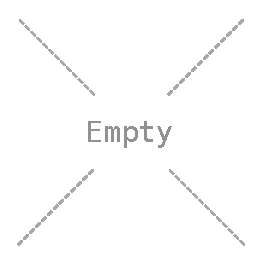
\includegraphics[height=\fgh]{empty.eps}
    }

    \mycaption{fig:usecase-battery}{Battery saver mode}{Energy-security tradeoff
    given strict energy budget as discussed in \cref{subsec:usecase-battery}.}
\end{figure}

 \hsg{we should exlude ChaCha8 only, unless
you have a major point here}

% About: result
\cref{fig:usecase-battery} shows the time versus energy used. At 0 seconds, we
begin writing. At 5 seconds, the ``battery saver'' event occurs, causing the
system to be underclocked. At 120 seconds, the system will die. If we blow past
our energy ceiling, the system will die. The figure shows two lines:
%
{\bf (1)} {\em Freestyle Balanced only}, that favors security even when backups
are paused; the device dies before the I/Os complete.
%
{\bf (2)} {\em Freestyle Balanced $+$ ChaCha8}, that performs the switch when
the system enters the low power state. Our results show that, while the system
uses slightly more power in the short term, we stay within our energy budget and
finish before the devices dies.
%
When we get the device to a charger (not shown), the cloud backup is enabled
again and when the nuggets are read, \sys automatically converges them back to
Freestyle Balanced.

% About: overall result
On average, using forward switching resulted in a 3.3x total energy reduction
compared to exclusively using Freestyle Balanced, allowing us to remain within
our energy budget. \hsg{I don't see this 3.3x in the graph. Did you accidentally
label the lines incorrectly?}. We note, however, that the energy savings is not
the point of this experiment. Rather, the lesson learned is that \sys enables
the system to move to the right point in the energy/security tradeoff space so
that the current task can still be accomplished before the battery is drained
and without compromising backup security at any point.


% ===============================
\subsection{No-Downtime Encryption Upgrade}\label{subsec:usecase-upgrade}

\def \hmina {\hspace{-0.1in}}
\def \hminb {\hspace{-0.2in}}

\def \fgw {2in}
\def \fgh {1in}

% \begin{floatingfigure}[r]{2in}  (and \end{..})

\begin{figure}[t]
    \centerline{
        % \hmina
        {\begin{tikzpicture}[baseline]

    \pgfmathsetmacro{\ymax}{15} % set the maximum y value
    \pgfmathsetmacro{\ymaxbreak}{15.1} % set the y value at which overflow is drawn

    \begin{axis}[
        %axis x line*=bottom,
        height=1in,
        width=2.5in,
        tick align=outside,
        tick pos=bottom, % make sure ticks only appear at the bottom and left axes
        tick style={ black },
        y tick label style={ /pgf/number format/fixed, /pgf/number format/precision=0 },
        grid style={ dotted, gray },
        every node near coord/.append style={font=\tiny},
        %
        % magic to make the numbers appear above the overly long bars:
        visualization depends on={rawy \as \rawy}, % save original y values
        restrict y to domain*={ % now clip/restrict any y value to ymax
            \pgfkeysvalueof{/pgfplots/ymin}:\ymaxbreak
        },
        after end axis/.code={ % draw squiggly line indicating break
            \draw [semithick, white, decoration={snake,amplitude=0.1mm,segment length=0.75mm,post length=0.375mm}, decorate] (rel axis cs:0,1.01) -- (rel axis cs:1,1.01);
        },
        nodes near coords={\color{.!75!black}\pgfmathprintnumber\rawy}, % print the original y values (darkened in case they are too light)...
        nodes near coords greater equal only=\ymax, % ... but ONLY if they are >= ymax
        clip=false, % allow clip to protrude beyond ymax
        % Custom stuff to edit per template
        %
        %xlabel={\scriptsize Cipher Configuration},
        xlabel near ticks,
        xmin=r, xmax=w,
        xtick=data,
        symbolic x coords={r,w},
        xticklabels={Read I/Os,Write I/Os},
        enlarge x limits=0.6, % add some breathing room along the x axis's sides
        %major x tick style=transparent,
        %
        ylabel={\scriptsize Latency (s)},
        ylabel near ticks,
        %ylabel shift={-1mm},
        ylabel style={at={(ticklabel cs:0.4)}},
        ymajorgrids=true,
        ymin=0, ymax=17,
        ybar, % value will shift bars
        ytick={ 5, 10, 15 },
        %yticklabels={ 5, 15, 25},
        % extra y ticks={1},
        % extra y tick style={grid=major, grid style={dashed, black}},
        % extra y tick label={\empty},
        %bar width=4.5pt, % change size of bars
        %
        legend cell align=center,
        legend style={ column sep=1ex },
        legend entries={
            {\scriptsize Pre-migration},
            {\scriptsize During migration},
            {\scriptsize Post-migration}
        },
        legend style={
            draw=none,
            legend columns=4,
            at={(0.5,1.02)},
            anchor=south,
        },
    ]
        \addplot[fill=redLight, every node near coord/.append style={color=redLight}]
        table[
            x=op,
            y=latency,
            col sep=space,
            discard if symbol not={stage}{pre}
        ] {data/usecase-upgrade.dat};
        \addplot[fill=purpleDark, every node near coord/.append style={color=purpleDark}]
        table[
            x=op,
            y=latency,
            col sep=space,
            discard if symbol not={stage}{dur}
        ] {data/usecase-upgrade.dat};
        \addplot[fill=blueDark, every node near coord/.append style={color=blueDark}]
        table[
            x=op,
            y=latency,
            col sep=space,
            discard if symbol not={stage}{post}
        ] {data/usecase-upgrade.dat};
    \end{axis}%
\end{tikzpicture}%
% \begin{tikzpicture}[baseline]
%     \begin{groupplot}[
%         % 6 seconds (0.3) + 3 seconds (0.15) + 11 seconds (0.55) = 1.0
%         no marks,
%         group style={
%             group size=1 by 2,
%             xlabels at=edge bottom,
%             ylabels at=edge left,
%             %xticklabels at=edge bottom,
%             yticklabels at=edge left,
%             vertical sep=35pt,
%             horizontal sep=15pt,
%         },
%         %axis x line*=bottom,
%         height=4cm,
%         width=\linewidth/1.25,
%         tick align=outside,
%         tick pos=bottom, % make sure ticks only appear at the bottom and left axes
%         title style={yshift=-1.5ex},
%         tick style={ black },
%         y tick label style={ /pgf/number format/fixed, /pgf/number format/precision=0 },
%         grid style={ dotted, gray },
%         point meta=explicit symbolic,
%         scatter/classes={
%             c8={mark=square*},
%             c20={mark=triangle*, red},
%             ff={mark=diamond*},
%             fb={mark=pentagon*},
%             fs={mark=otimes, red}
%         },
%         %every node near coord/.append style={font=\tiny},
%         %
%         % magic to make the numbers appear above the overly long bars:
%         % visualization depends on={rawy \as \rawy}, % save original y values
%         % restrict y to domain*={ % now clip/restrict any y value to ymax
%         %     \pgfkeysvalueof{/pgfplots/ymin}:\ymaxbreak
%         % },
%         % after end axis/.code={ % draw squiggly line indicating break
%         %     \draw [semithick, white, decoration={snake,amplitude=0.1mm,segment length=0.75mm,post length=0.375mm}, decorate] (rel axis cs:0,1.01) -- (rel axis cs:1,1.01);
%         % },
%         % nodes near coords={\color{.!75!black}\pgfmathprintnumber\rawy}, % print the original y values (darkened in case they are too light)...
%         % nodes near coords greater equal only=\ymax, % ... but ONLY if they are >= ymax
%         % clip=false, % allow clip to protrude beyond ymax
%         % Custom stuff to edit per template
%         %
%         xlabel near ticks,
%         xlabel shift={-0.5mm},
%         xmin=0, xmax=1,
%         %enlarge x limits=0.2, % add some breathing room along the x axis's sides
%         %
%         ylabel near ticks,
%         %ylabel shift={-1.5mm},
%         ymajorgrids=false,
%         ymin=0, ymax=4,
%         ytick={ 0, 1, 1.5, 2, 3, 4 },
%         yticklabels={ 0,,0.5,, 1, \empty },
%         major y tick style=transparent,
%         %yticklabels={ 0, 0.5, 1.5, 2 },
%         % extra y ticks={1},
%         % extra y tick style={grid=major, grid style={dashed, black}},
%         % extra y tick label={\empty},
%         %bar width=4.5pt, % change size of bars
%         %
%         legend cell align=center,
%         legend style={ column sep=1ex },
%         legend entries={%
%             {\scriptsize Mirrored Scores (no switching)},
%             {\scriptsize Desired Minimum Score},
%             {\scriptsize Actual Minimum Score (switching)}
%         },
%         legend style={
%             draw=none,
%             legend columns=2,
%             at={(0.5,1.2)},
%             anchor=south,
%         },
%     ]
%         \nextgroupplot[
%             xlabel={\scriptsize Time (s)},
%             ylabel={\scriptsize Trade Score},
%             xtick={ 0, 0.3, 0.45, 1 },
%             xticklabels={ 0, 6, 9, \ldots },
%         ]
%             \addplot [thick, red] table [
%                 x=time,
%                 y=score,
%                 discard if number not={line}{1},
%                 col sep=space
%             ] {data/usecase-upgrade.dat};
%             \addplot [thick, red, forget plot] table [
%                 x=time,
%                 y=score,
%                 discard if number not={line}{3},
%                 col sep=space
%                 ] {data/usecase-upgrade.dat};
%             \addplot [thick, densely dotted, blue] table [
%                 x=time,
%                 y=score,
%                 discard if number not={line}{2},
%                 col sep=space
%                 ] {data/usecase-upgrade.dat};
%             \addplot [thick, dashed, blue] table [
%                 x=time,
%                 y=score,
%                 discard if number not={line}{4},
%                 col sep=space,
%                 ] {data/usecase-upgrade.dat};
%             \coordinate (c1) at (0.375, 3.5);
%             \coordinate (c2) at (0.415, 3.5);
%             \draw [dotted, black] (0.2945, 0) -- (0.2945, 4) node [left of=c1] {\tiny (panic; ISE)};
%             \draw [dotted, black] (0.455, 0) -- (0.455, 4) node [right of=c2] {\tiny (ISE completes)};
%         \nextgroupplot[
%             scatter,
%             legend to name={throwaway8},
%             xlabel={\scriptsize Latency (norm)},
%             ylabel={\scriptsize Trade Score},
%             xtick={ 0, 1 },
%             xticklabels={ 0, 1 },
%         ]
%             \addplot [thick] table [
%                 meta=cipher,
%                 x=latency,
%                 y=score,
%                 discard if symbol not={iop}{40m-r},
%                 discard if symbol not={order}{seq},
%                 col sep=space
%             ] {data/tradeoff-baseline.dat};
%             \coordinate (c3) at (0.27, 1.75);
%             \coordinate (c4) at (0.755, 0.5);
%             \draw [dotted] (0.035, 0) -- (0.035, 4) node [above of=c3] {\tiny (pre-panic latency ceiling)};
%             \draw [dotted] (0.999, 0) -- (0.999, 4) node [above of=c4] {\tiny (post-panic latency ceiling)};
%     \end{groupplot}%
% \end{tikzpicture}%
}
        % \hminb
        %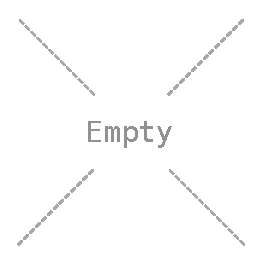
\includegraphics[height=\fgh]{empty.eps}
    }

    \mycaption{fig:usecase-upgrade}{No-downtime encryption upgrade}{Upgrading
    storage system encryption with zero downtime as discussed in
    \cref{subsec:usecase-upgrade}.}
\end{figure}


In \cref{fig:usecase-upgrade} \TODO{finish sentence}. \hsg{we must have a short
case study here. Otherwise no point of talking about mirrored switch}.


% ================================================================
\subsection{Select Data Encryption}\label{subsec:usecase-agnostic}

% About: background
This case study illustrates utility of selective switching to achieve a
performance win---if only a small percentage of the data needs the strongest
encryption, then only a small percentage of the data should have that associated
overhead, while the rest can use a minimalist encryption. As mentioned before,
this feature requires users to annotate certain files with a special tag via
file system calls, which would then be stored in the inode. Because the \sys
layer is file oblivious, every block I/O through the \sys layer will be labeled
with the corresponding cipher.

% About: setup
We begin by with 10 5MB and 4KB write-read operations to two \sys drive
instances: one using ChaCha8 and the other using Freestyle Strong. They
represent two extreme where ChaCha8 is a low-latency cipher and Freestyle Strong
exhibits a very high overhead. We then run another \sys instance with a 7:3
ratio where 30\% of the data considered highly sensitive uses Freestyle Strong.

\def \hmina {\hspace{-0.1in}}
\def \hminb {\hspace{-0.2in}}

\def \fgw {2in}
\def \fgh {1in}

% \begin{floatingfigure}[r]{2in}  (and \end{..})

\begin{figure}[t]
    \centerline{
        % \hmina
        {\begin{tikzpicture}[baseline]

    \pgfmathsetmacro{\ymax}{20} % set the maximum y value
    \pgfmathsetmacro{\ymaxbreak}{20.1} % set the y value at which overflow is drawn

    \begin{axis}[
        %axis x line*=bottom,
        height=1in,
        width=2.5in,
        tick align=outside,
        tick pos=bottom, % make sure ticks only appear at the bottom and left axes
        tick style={ black },
        y tick label style={ /pgf/number format/fixed, /pgf/number format/precision=0 },
        grid style={ dotted, gray },
        every node near coord/.append style={font=\tiny},
        %
        % magic to make the numbers appear above the overly long bars:
        visualization depends on={rawy \as \rawy}, % save original y values
        restrict y to domain*={ % now clip/restrict any y value to ymax
            \pgfkeysvalueof{/pgfplots/ymin}:\ymaxbreak
        },
        after end axis/.code={ % draw squiggly line indicating break
            \draw [semithick, white, decoration={snake,amplitude=0.1mm,segment length=0.75mm,post length=0.375mm}, decorate] (rel axis cs:0,1.01) -- (rel axis cs:1,1.01);
        },
        nodes near coords={\color{.!75!black}\pgfmathprintnumber\rawy}, % print the original y values (darkened in case they are too light)...
        nodes near coords greater equal only=\ymax, % ... but ONLY if they are >= ymax
        clip=false, % allow clip to protrude beyond ymax
        % Custom stuff to edit per template
        %
        xlabel={\scriptsize Cipher Configuration},
        xlabel near ticks,
        xmin=C8+FS, xmax=FS,
        xtick=data,
        symbolic x coords={C8+FS,FS},
        xticklabels={Selective (C8+FS),FS only},
        enlarge x limits=0.5, % add some breathing room along the x axis's sides
        %major x tick style=transparent,
        %
        ylabel={\scriptsize Latency (s)},
        ylabel near ticks,
        %ylabel shift={-1mm},
        ylabel style={at={(ticklabel cs:0.4)}},
        ymajorgrids=true,
        ymin=0, ymax=30,
        ybar, % value will shift bars
        ytick={ 5, 15, 25 },
        %yticklabels={ 5, 15, 25},
        % extra y ticks={1},
        % extra y tick style={grid=major, grid style={dashed, black}},
        % extra y tick label={\empty},
        %bar width=4.5pt, % change size of bars
        %
        legend cell align=center,
        legend style={ column sep=1ex },
        legend entries={
            {\scriptsize 4K/reads},
            {\scriptsize 4K/writes},
            {\scriptsize 5M/reads},
            {\scriptsize 5M/writes},
        },
        legend style={
            draw=none,
            legend columns=4,
            at={(0.5,1.02)},
            anchor=south,
        },
    ]
        \addplot[fill=pinkDark, every node near coord/.append style={color=pinkDark}]
        table[x=conf, y=latr-4k, col sep=space] {data/usecase-agnostic.dat};
        \addplot[fill=pinkDark, postaction={pattern=north east lines}, every node near coord/.append style={color=purpleDark}]
        table[x=conf, y=latw-4k, col sep=space] {data/usecase-agnostic.dat};
        \addplot[fill=purpleDark, every node near coord/.append style={color=pinkDark}]
        table[x=conf, y=latr-5m, col sep=space] {data/usecase-agnostic.dat};
        \addplot[fill=purpleDark, postaction={pattern=north east lines}, every node near coord/.append style={color=purpleDark}]
        table[x=conf, y=latw-5m, col sep=space] {data/usecase-agnostic.dat};
    \end{axis}%
\end{tikzpicture}%
}
        % \hminb
        %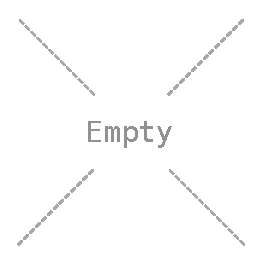
\includegraphics[height=\fgh]{empty.eps}
    }

    \mycaption{fig:usecase-agnostic}{Scalable encryption}{Filesystem-agnostic
    file-level encryption as discussed in \cref{subsec:usecase-agnostic}.}
\end{figure}


% About: outcome
The left-side and right-side bars in \cref{fig:usecase-agnostic} show the two
extremes; ChaCha8 exhibits a low latency, consistently less than 1 second across
the workloads, while Freestyle Strong exhibits 5 to 20 second latency depending
on the workload. The selective switching (middle bars) shows a reduction of 3.1x
to 4.8x for read latency and 1.6x to 2.8x for write latency, all without
compromising the security needs of the most sensitive data. Thus, selective
switching keeps our sensitive data at the mandated security level while keeping
the performance (and also battery life) benefits of using a fast cipher for the
majority of I/O operations.
